\graphicspath{{./third/img/}}
\lstdefinelanguage{Dockerfile}
{
  morekeywords={FROM, RUN, CMD, LABEL, MAINTAINER, EXPOSE, ENV, ADD, COPY,
    ENTRYPOINT, VOLUME, USER, WORKDIR, ARG, ONBUILD, STOPSIGNAL, HEALTHCHECK,
    SHELL},
  morecomment=[l]{\#},
  morestring=[b]"
}

\section*{\LARGE Введение}
\addcontentsline{toc}{section}{Введение}
Docker~--- это платформа, которая предназначена для разработки,
развёртывания и запуска приложений в контейнерах.
Слово "<Docker"> в последнее время стало чем-то вроде синонима слова
"<контейнеризация">. И если вы ещё не пользуетесь Docker, но при этом
работаете или собираетесь работать в сферах разработки приложений или
анализа данных, то Docker~--- это то, с чем вы непременно встретитесь
в будущем.

\clearpage

\section{Образы}
Посмотрели на имеющиеся образы: \texttt{docker~images}.
Загрузив образ: \texttt{docker~pull~ubuntu} --- будет загружен образ
\textit{ubuntu:latest} --- последняя доступная версия.
Для загрузки конкретной версии, нужно указать тег, например, 12.04:
\texttt{docker~pull~ubuntu:12.04}. Посмотрели на имеющиеся образы ещё раз:
\texttt{docker~images} --- появились новые загруженные
образы. Теперь можно просмотреть список контейнеров,
выполнив команду: \texttt{docker~ps~-a}.\par
Пример проиллюстрирован на рисунке~\ref{fig:images}.

\begin{image}
	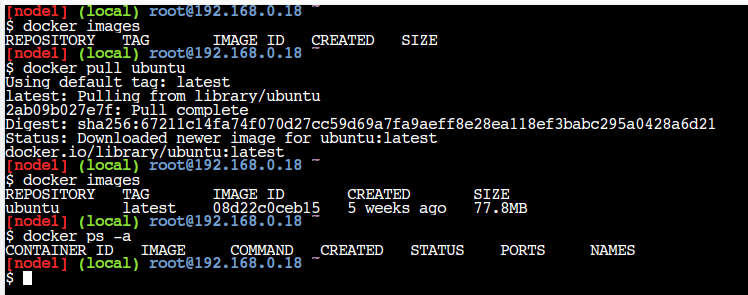
\includegraphics[width=1\textwidth]{Screenshot from 2023-04-15 15-17-36}
	\caption{Загрузка образа Ubuntu}
	\label{fig:images}
\end{image}

\section{Изоляция}
\textbf{Вопрос:} одинаковый ли результат получился при разных запусках?\par
\textbf{Ответ:} да, результат одинаковый, так как команда hostname выводит имя
хоста, которое задано в системе.\par
Запуск контейнеров производится командой:

Запуск контейнеров производится командой:

\begin{verbatim}
docker run --флаги --докера имя_контейнера команда для запуска
	-и --флаги --запуска --программы.
\end{verbatim}

Если запустить bash в контейнере командой: \texttt{docker~run~ubuntu~bash},
ничего не произойдет. Интерактивные оболочки выйдут после
выполнения любых скриптовых команд, если только они не будут
запущены в интерактивном терминале --- поэтому для того, чтобы этот пример
не завершился, нужно добавить флаги \texttt{-i~-t}
или сгруппированно \texttt{-it}: \texttt{docker~run~-it~ubuntu~bash}.
Выполняя запуск контейнера, указывая образ ubuntu,
неявно указывался образ \textit{ubuntu:latest}.
Следовательно, следующие команды равнозначны:

\begin{itemize}
	\item \texttt{docker run ubuntu hostname};
	\item \texttt{docker run ubuntu:latest hostname}.
\end{itemize}

\textbf{Вопрос:} Одинаковый ли результат получился при разных запусках?\par
\textbf{Ответ:} нет, результат разный, Так происходит, потому что из одного
образа ubuntu были запущены два изолированных контейнера, поэтому у
них и был разный hostname.\par
Если нужно запустить ubuntu:12.04, то надо выполнить команду
\texttt{docker run ubuntu:12.04 hostname}.\par
Пример проиллюстрирован на рисунке~\ref{fig:run}.

\begin{image}
	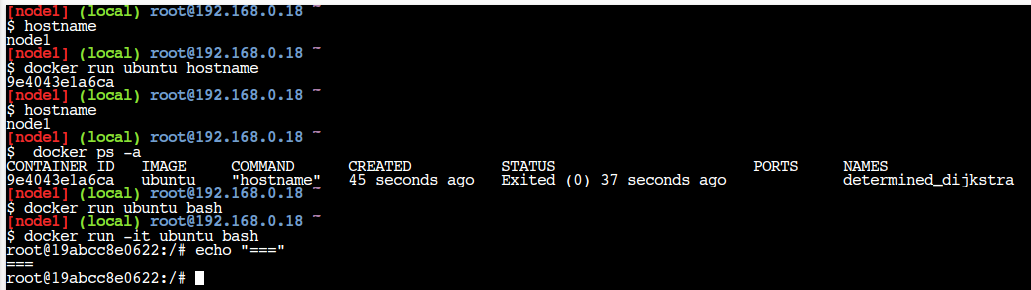
\includegraphics[width=1\textwidth]{Screenshot from 2023-04-15 15-31-58}
	\caption{Взаимодействие с контейнером}
	\label{fig:run}
\end{image}

\section{Работа с портами}
Для начала, загрузили образ python командой \texttt{docker pull python}.\par
В качестве примера, запустили встроенный в Python модуль веб-сервера
из корня контейнера, чтобы отобразить содержание контейнера:
\texttt{docker run -it python python -m http.server}\par
При запуске пишется, что сервер доступен по адресу
\textit{http://0.0.0.0:8000/}. Однако, если открыть этот адрес,
то ничего не будет видно, потому что порты не проброшены.
Тогда завершили работу веб-сервера, нажав комбинацию клавиш
\texttt{Ctrl+C}.\par
Для проброса портов используется флаг \texttt{-p~hostPort:containerPort}\par
Добавили его, чтобы пробросить порт 8000:
\texttt{docker~run~-it~-p8000:8000~python~python~-m~http.server}~--- теперь
по адресу http://0.0.0.0:8000/ открывается содержимое корневой директории
в контейнере.\par
Для того, чтобы доступный в контейнере на порту 8000 веб-сайт
в хостовой системе открывался на порту 8888, необходимо указать флаг
\texttt{-p~8888:8000}:
\texttt{docker~run~-it~-p8888:8000~python~python~-m~http.server}.\par
Завершили работу веб-сервера, нажав комбинацию клавиш Ctrl+C.
Пример проиллюстрирован на рисунке~\ref{fig:server}.

\begin{image}
	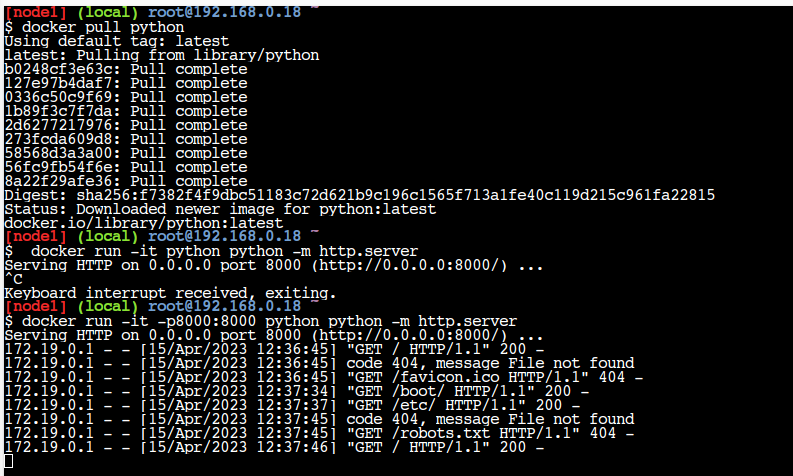
\includegraphics[width=1\textwidth]{Screenshot from 2023-04-15 15-38-00}
	\caption{Указание портов для доступа к серверу}
	\label{fig:server}
\end{image}

\section{Именованные контейнеры, остановка и удаление}
Запустили контейнер:
\texttt{docker run -it -p8000:8000 python python -m http.server}.
Нажав \texttt{Ctrl+C} --- выполнение завершится.
Для того, чтобы запустить контейнер в фоне, нужно добавить флаг
\verb|-d/--detach|.
Также определили имя контейнеру, добавив флаг \verb|--name|.

\begin{verbatim}
docker run -p8000:8000 --name pyserver -d python python -m http.server
\end{verbatim}

Для того, чтобы остановить выполнение контейнера, существует команда
\texttt{docker stop pyserver}. Однако, если снова попробовать запустить
командой \texttt{docker run -it -p8000:8000 --name pyserver -d python
python -m http.server}, то возникнет ошибка:
\textit{контейнер с таким именем существует}.
Его нужно удалить \texttt{docker rm pyserver}.\par
Для остановки и удаления контейнера можно воспользоваться командой
\texttt{docker rm -f pyserver} вместо выполнения двух отдельных команд
\texttt{stop} и \texttt{rm}. После удаления контейнер с таким именем можно
будет создать заново.\par
Для того, чтобы контейнер удалялся после завершения работы, нужно указать
флаг \verb|--rm| при его запуске -- далее в работе мы будем использовать
данный флаг:

\begin{verbatim}
docker run --rm -p8000:8000 --name pyserver -d python
	python -m http.server
\end{verbatim}

Пример проиллюстрирован на рисунке~\ref{fig:rm:stop}.

\begin{image}
	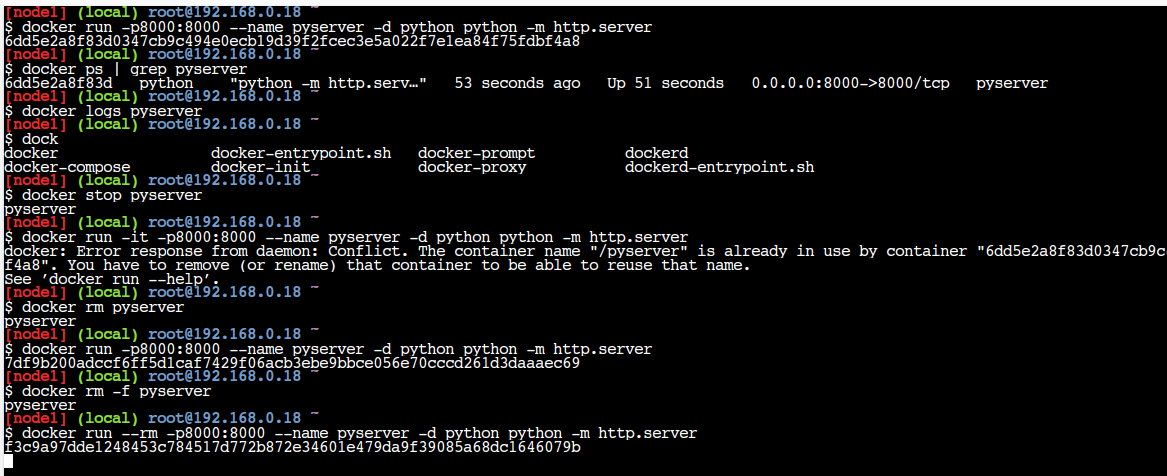
\includegraphics[width=1\textwidth]{Screenshot from 2023-04-15 15-46-04}
	\caption{Остановака и удаление именованных контейнеров}
	\label{fig:rm:stop}
\end{image}

\section{Постоянное хранение данных}
Запустили контейнер, в котором веб-сервер будет отдавать
содержимое директории /mnt:

\begin{verbatim}
docker run -p8000:8000 --name pyserver --rm -d python python -m
	http.server -d /mnt
\end{verbatim}

\textbf{Вопрос:} Что значат остальные флаги запуска? Где здесь команда,
которая выполнится в контейнере?\par

\begin{itemize}
	\item "<-p8000:8000"> - пробрасывает порт 8000 из контейнера на порт
		8000 хост-машины, чтобы веб-сервер был доступен по адресу
		http://localhost:8000.
	\item "<-name pyserver"> - задает имя контейнеру, которое может
		использоваться для его идентификации вместо автоматически
		генерируемого имени.
	\item "<-rm"> - удаляет контейнер после остановки.
	\item "<-d"> - запускает контейнер в фоновом режиме.
	\item "<python python -m http.server -d /mnt"> - это команда,
		которая выполнится внутри контейнера. Она запустит веб-сервер
		на порту 8000 и указывает директорию /mnt как корневую
		для отображения содержимого.
\end{itemize}

Где \texttt{-d /mnt} указывает модулю
\texttt{http.server} какая директория будет корневой для отображения.
Для того, чтобы попасть в уже запущенный контейнер,
существует команда \texttt{docker exec -it pyserver bash} --- попали
в оболочку bash в контейнере. Попав в контейнер, выполнили команду
\verb|cd mnt && echo "hello world" > hi.txt|, а затем выйшли из контейнера,
введя команду \texttt{exit} или нажав комбинацию клавиш \texttt{Ctrl+D}.\par
Если открыть \textit{http://0.0.0.0:8000/},
там будет доступен файл hi.txt.\par
Остановили контейнер: \texttt{docker stop pyserver}, а затем снова запустили:

\begin{verbatim}
docker run -p8000:8000 --name pyserver --rm -d python python -m
	http.server -d /mnt
\end{verbatim}

Увидели, что файл hi.txt пропал --- это неудивительно, был запущен
другой контейнер, а старый был удалён после завершения работы
(флаг \verb|--rm|).
Остановили контейнер: \texttt{docker stop pyserver}.
Для того, чтобы не терялись какие-то данные
(например, если запущен контейнер с СУБД, то чтобы
не терялись данные из неё) существует механизм монтирования.\par
Пример проиллюстрирован на рисунке~\ref{fig:storage}.

\begin{image}
	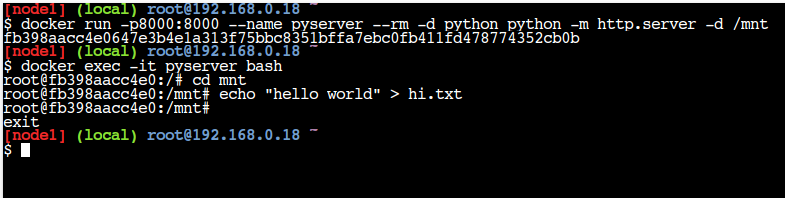
\includegraphics[width=1\textwidth]{Screenshot from 2023-04-15 15-51-10}
	\caption{Попытка хранения данных}
	\label{fig:storage}
\end{image}

\subsection{Тома}
Первый способ --- это создать отдельный том с помощью ключа
\texttt{-v myvolume:/mnt}, где myvolume --- название тома,
/mnt --- директория в контейнере, где будут доступны данные.\par
Попробовали снова создать контейнер, но уже с примонтированным томом:

\begin{verbatim}
docker run -p8000:8000 --rm --name pyserver -d -v $(pwd)/myfiles:/mnt python
	python -m http.server -d /mnt
\end{verbatim}

Затем, если создать файл (выполнить \texttt{docker exec -it pyserver bash}
и внутри контейнера выполнить \verb|cd mnt && echo "hello world" > hi.txt|),
то даже после удаления контейнера данные в этом томе будут сохранены.\par
Пример проиллюстрирован на рисунке~\ref{fig:tom}.

\begin{image}
	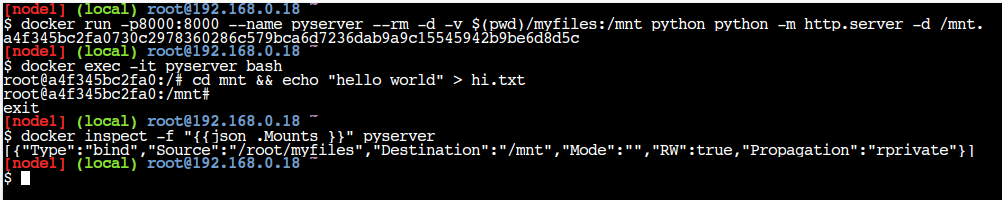
\includegraphics[width=1\textwidth]{Screenshot from 2023-04-15 16-13-18}
	\caption{Использование томов}
	\label{fig:tom}
\end{image}

\subsection{Монтирование директорий и файлов}
Иногда требуется пробросить в контейнер конфигурационный файл
или отдельную директорию. Для этого используется монтирование директорий
и файлов.\par
Создали директорию и файлы, которые будем монтировать.
Часть из них понадобится дальше: создали директорию:
\texttt{mkdir myfiles}, в ней создали файл \texttt{host.txt}:
\texttt{touch myfiles/host.txt}\par
Запустили контейнер:

\begin{verbatim}
docker run -p8000:8000 --rm --name pyserver -d -v $(pwd)/myfiles:/mnt python \
	python -m http.server -d /mnt
\end{verbatim}

Команда \texttt{pwd} --- выведет текущую директорию.
В итоге получился абсолютный путь до файла.
Обратный слеш (\textbackslash) перед переводом строки экранирует символ
перевода строки и позволяет написать одну команду в несколько строк.\par
Затем, зайшли в контейнер: \texttt{docker exec -it pyserver bash},
перешли в директорию /mnt командой \texttt{cd /mnt}.
Если вывести список файлов командой \texttt{ls}, то там будет файл host.txt,
примонтированный вместе с директорией myfiles.\par
Создали файл \verb|echo "hello world" > hi.txt|, а затем выйшли
из контейнера. Теперь на хостовой машине в директории myfiles/ появится файл
hi.txt. Проверить можно командой \texttt{ls myfiles}, как
показано на рисунке~\ref{fig:mount:out}.\par

\begin{image}
	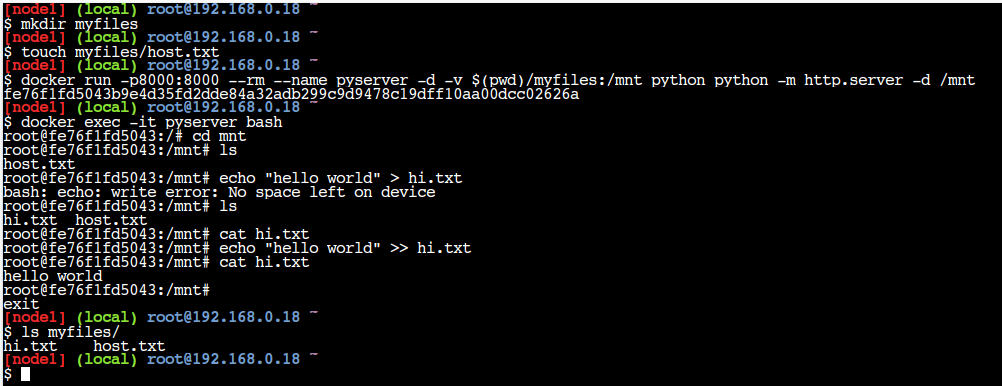
\includegraphics[width=1\textwidth]{Screenshot from 2023-04-15 16-21-54}
	\caption{Примонтирование директории}
	\label{fig:mount:out}
\end{image}

Для того, чтобы примонтировать один файл, нужно указать ключ \texttt{-v},
например:
\verb|-v $(pwd)/myfiles/host.txt:/mnt/new-name-of-host.txt|~--- файлу
в контейнере присвоится другое имя: new-name-of-host.txt
(Рисунок~\ref{fig:mount:in}).

\begin{image}
	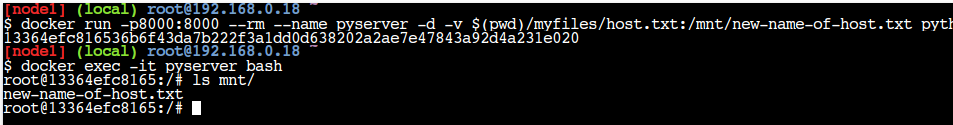
\includegraphics[width=1\textwidth]{Screenshot from 2023-04-15 16-24-49}
	\caption{Примонтирование директории}
	\label{fig:mount:in}
\end{image}

\section{Переменные окружения}
Для передачи переменных окружения внутрь контейнера используется ключ
\texttt{-e}. Например, чтобы передать в контейнер переменную окружения
\texttt{MIREA} во значением \texttt{"<ONE~LOVE">}, нужно добавить
ключ: \texttt{-e~MIREA="ONE~LOVE"}.\par
Проверили, выведя все переменные окружения, определённые в контейнере
с помощью утилиты env:

\begin{verbatim}
docker run -it --rm -e MIREA="ONE~LOVE" ubuntu env
\end{verbatim}

Среди списка переменных будет и \texttt{MIREA}.
Пример проиллюстрирован на рисунке~\ref{fig:env}.

\begin{image}
	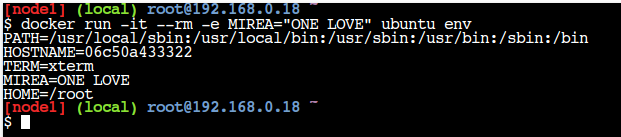
\includegraphics[width=1\textwidth]{Screenshot from 2023-04-15 16-26-19}
	\caption{Манипулирование переменными окружения}
	\label{fig:env}
\end{image}

\section{Dockerfile}
Собрали образ, в котором установлены дополнительные пакеты,
примонтировали директорию и установили команду запуска.
Для этого создаётся файл Dockerfile.

\begin{lstlisting}[language=Dockerfile
	, caption=\leftline{Код Dockerfile-а}
	, label=lst:dockerfile]
FROM ubuntu:20.04
RUN apt update \
	&& apt install -y zip \
	&& apt install -y python3 \
	&& cd /usr/bin \
	&& ln -s python3 python
ADD ./data /mnt/files/ 
EXPOSE 80
CMD ["python" , "-m" , "http.server" , "-d" , "/mnt/" , "80"]
\end{lstlisting}

Затем собрали образ с тегом mycoolimage с помощью команды
\texttt{docker build -t mycoolimage .}, где точка в конце указывает
на текущую директорию, где лежит Dockerfile.\par
Запуск производится командой:

\begin{verbatim}
docker run --rm -it -p8099:80 mycoolimage
\end{verbatim}

Где порт 8099 --- порт
на хостовой машине.\par
Пример проиллюстрирован
на рисунках~\ref{fig:dockerfile}\,-\,\ref{fig:dockerfile:run}.

\begin{image}
	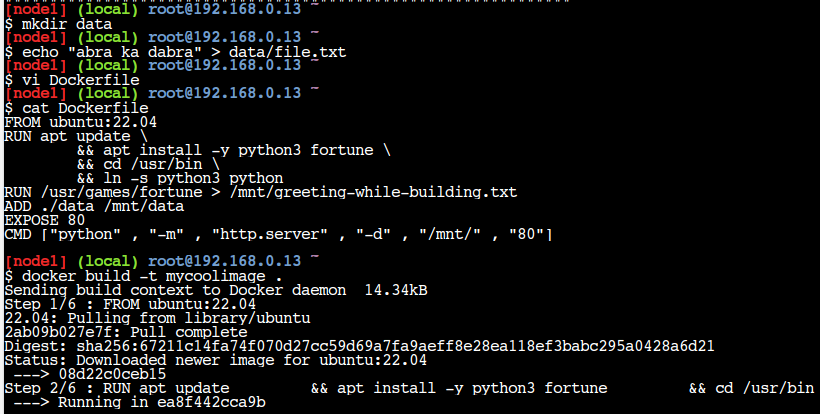
\includegraphics[width=1\textwidth]{Screenshot from 2023-04-15 21-07-19}
	\caption{Использование Dockerfile}
	\label{fig:dockerfile}
\end{image}

\begin{image}
	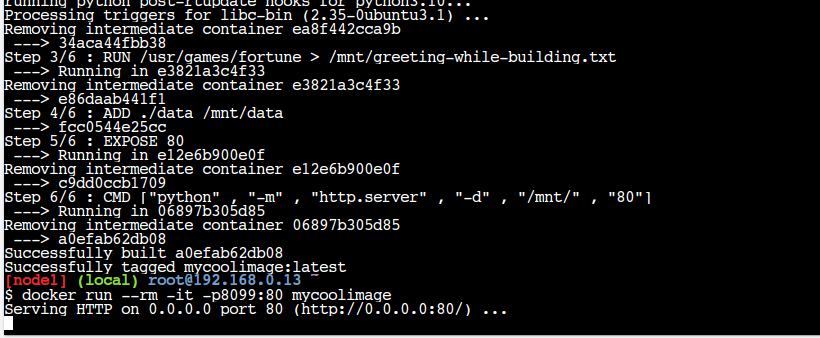
\includegraphics[width=1\textwidth]{Screenshot from 2023-04-15 21-08-59}
	\caption{Использование Dockerfile}
	\label{fig:dockerfile:run}
\end{image}

\section{Индивидуальные задания}
Индивидуальное задание заключается в написании Dockerfile-а,
соборки образа и запуске контейнер
(и записи команды для его запуска).\par
Для монтирования создали директорию data и в ней файл student.txt,
содержащий ФИО, название группы и номер варианта (третий).\par
Для установки пакетов использовали команду
\texttt{apt install -y название-пакета}.\par
Также условия заключались в необходимости использовать
базовый образ \textit{ubuntu:20.04}
и примонтировать директорию data в директорию /mnt/files/ в контейнере.
Запустить веб-сервер, отображающий содержимое /mnt/files, в хостовой
системе должен открываться на порту (8800 + номер варианта).
В данном случае использовался порт 8803.\par
И установить пакет zip, согласно варианту.\par
Реализация проиллюстрирована
на рисунках~\ref{fig:indvar}\,-\,\ref{fig:indvar:page}.

\begin{image}
	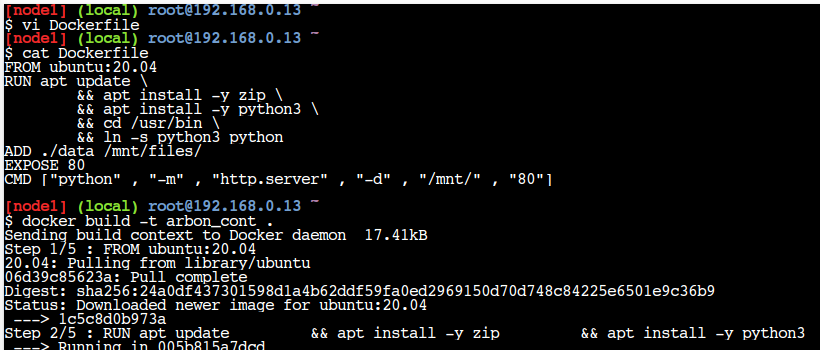
\includegraphics[width=1\textwidth]{Screenshot from 2023-04-15 21-24-51}
	\caption{Выполнение индивидуального варианта}
	\label{fig:indvar}
\end{image}

\begin{image}
	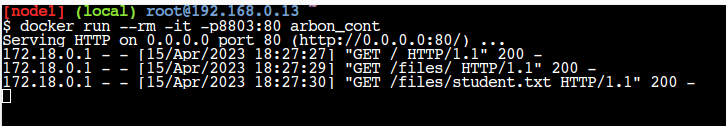
\includegraphics[width=1\textwidth]{Screenshot from 2023-04-15 21-27-55}
	\caption{Выполнение индивидуального варианта}
	\label{fig:indvar:run}
\end{image}

\begin{image}
	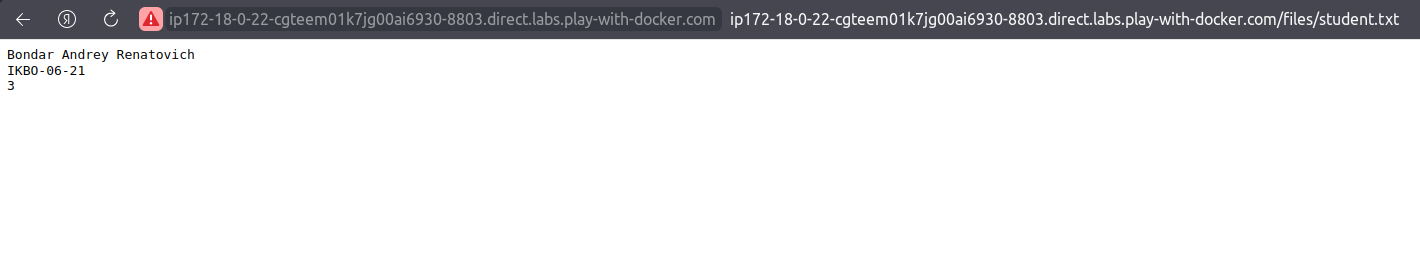
\includegraphics[width=1\textwidth]{Screenshot from 2023-04-15 21-27-44}
	\caption{Страница запущенного сервера}
	\label{fig:indvar:page}
\end{image}

\clearpage

\section*{\LARGE Выводы}
\addcontentsline{toc}{section}{Выводы}
В данной практической работе научились писать базовые команды Docker-а,
например как: загрузка имеющихся образов, запуск контейнера, проброска
портов или запуск команды в контейнере.\par
Также научились упарвлять контейнера, создавать тома и примонтировать
директории. И писать скрипты в Dockerfile.

